\documentclass[a4paper,11pt,notitlepage]{article}
\usepackage{amsmath}
\usepackage{amsfonts}
\usepackage{amssymb}
\usepackage[UTF8]{ctex}
\usepackage{graphicx}
\usepackage{color}
\usepackage{changepage}
\usepackage{enumitem}
\usepackage{subfigure}
\usepackage{float}
\usepackage[backend=biber]{biblatex}

\usepackage{titlesec}
\titleformat{\section}{\bfseries\Large}{$\S$\,\thesection}{1em}{}
\titleformat{\subsection}{\bfseries\large}{\Roman{subsection}}{1em}{}
\titleformat{\subsubsection}{\bfseries\normalsize}{\roman{subsubsection}}{1em}{}
\titlespacing*{\subsection}{2em}{2pt}{2pt}
\titlespacing*{\subsubsection}{3em}{2pt}{2pt}
\title{\vspace{-1.5cm} \textbf{\huge{数值分析第10章上机}}\vspace{-1em}}
\author{By 211870125 陈睿硕}
\date{}

\usepackage{geometry}
\geometry{left=2cm,right=2cm,top=2cm,bottom=2cm}

\usepackage{fancyhdr}
\pagestyle{fancy}
\fancyhf{}
\fancyhead[L]{Chapter 10}
\fancyhead[R]{\thepage}
\setlength{\headheight}{14pt}

\definecolor{darkgreen}{RGB}{0,150,0}

\usepackage{listings}  % 引入 listings 包
\lstset{                % 定义代码块的样式
    basicstyle=\normalsize\ttfamily, % 设定代码字体大小、样式
    showspaces=false,   % 不显示空格
    showstringspaces=false, % 不显示字符串中的空格
    showtabs=false,     % 不显示制表符
    frame=single,       % 设定代码块边框样式
    rulecolor=\color{black}, % 设定代码块边框颜色
    tabsize=4,          % 设定制表符长度为 4 个字符
    captionpos=t,       % 设定标题位置为底部
    keywordstyle=\bfseries\color{blue}\ttfamily,
    stringstyle=\color{red}\ttfamily,
    commentstyle=\color{darkgreen}\ttfamily,
    morecomment=[l][\color{magenta}]{\#},
    framesep=0.5em,
    frameround=tttt,
    breaklines=true,    % 自动换行
    breakatwhitespace=false, % 只在空格分割处换行
    escapeinside={\%*}{*)}   % 允许使用 LaTeX 命令
}
\renewcommand{\lstlistingname}{代码}

\usepackage{hyperref}
\usepackage{cleveref}
\crefname{theorem}{定理}{定理}
\crefname{figure}{图}{图}
\crefname{equation}{式}{式}
\crefname{listing}{代码}{代码}
\crefname{table}{表}{表}

\begin{document}
\maketitle
\vspace{-1cm}
\thispagestyle{fancy}

\section{问题}
\begin{adjustwidth}{1em}{0pt}
    对于常微分方程初值问题:
    \[    
    \begin{cases}
            y'=-\frac{1}{x^2}-\frac{y}{x}-y^2,1\leqslant x\leqslant 2,\\
            y(1)=-1.
    \end{cases}
    \]
\begin{enumerate}[label=\textbf{Q\arabic*}]
    \item 分别用Euler方法、改进的Euler方法、Heun公式、中点方法和四阶Runge-Kutta方法求解上述初值问题,
    列表、画图比较他们的计算结果。\label{Q1}\notag
    \item 用经典的Runge-Kutta方法提供初始出发值,与四阶Adams预测-校正方法
    的PECE模式结合起来求解上述初值问题,并与\ref{Q1}中的四阶Runge-Kutta方
    法求解进行比较。\label{Q2}\notag
\end{enumerate}
\end{adjustwidth}

\section{算法思路}
\subsection{对\ref{Q1},\ref{Q2}的解答}
使用python实现,代码见\cref{code1}。计算出初值问题的精确解为:$y=(x \tan(\ln(x)-\frac{\pi}{4}))^{-1}$。
取$h=0.0001$,得到误差(绝对值)和x的关系如\cref{pic:1}。
\begin{figure}[H]
    \centering
    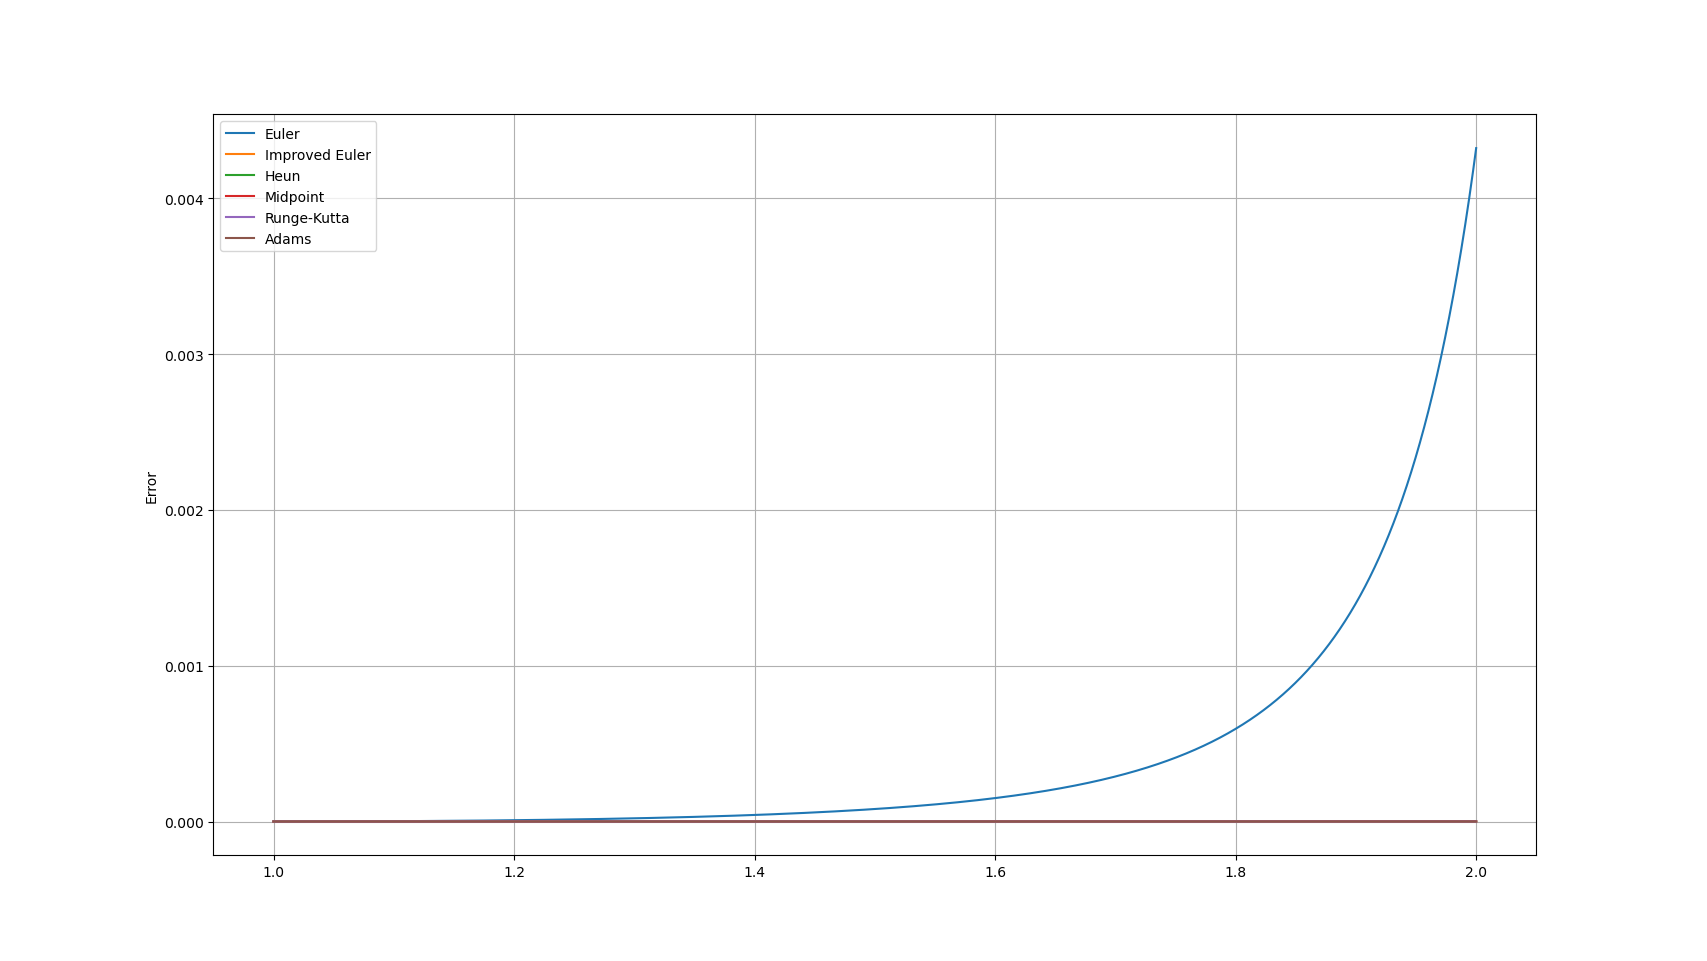
\includegraphics[width=0.8\textwidth]{../picture/Tenth_Chapter.png}
    \caption{误差(绝对值)和x的关系}
    \label{pic:1}
\end{figure}
得到x=2处的误差如\cref{tab:1}。
\begin{table}[ht]
    \begin{center}
    \begin{tabular}{|c|c|}
        \hline
        Method & Error \\
        \hline
        Euler方法 & 0.004321987481701761 \\
        \hline
        改进的Euler方法 & 4.807119715621866e-07 \\
        \hline
        Heun公式 & 7.116845477384004e-07 \\
        \hline
        中点方法 & 8.271718101582337e-07 \\
        \hline
        四阶Runge-Kutta方法 & 3.0047075938455237e-12\\
        \hline
        Adams方法&3.375077994860476e-12\\
        \hline
        \end{tabular}
        \caption{x=2处的误差}
        \label{tab:1}
    \end{center}
\end{table}

\section{附录:程序代码}
\begin{lstlisting}[language=Python,caption={Tenth Chapter.py},label={code1}]
import numpy as np
from matplotlib import pyplot as plt

def y(x):
    return 1/(x*np.tan(np.log(x)-np.pi/4))


h = 0.0001
x = np.arange(1, 2+h, h)
y0 = -1


def f(x, y):
    return -1/x**2 - y/x - y**2


def euler(x, y0, f):
    y = np.zeros(x.shape)
    y[0] = y0
    for i in range(len(x) - 1):
        y[i+1] = y[i] + h * f(x[i], y[i])
    return y


def improved_euler(x, y0, f):
    y = np.zeros(x.shape)
    y[0] = y0
    for i in range(len(x) - 1):
        k1 = f(x[i], y[i])
        k2 = f(x[i+1], y[i] + h * k1)
        y[i+1] = y[i] + h * (k1 + k2) / 2
    return y


def heun(x, y0, f):
    y = np.zeros(x.shape)
    y[0] = y0
    for i in range(len(x) - 1):
        k1 = f(x[i], y[i])
        k2 = f(x[i] + 2*h/3, y[i] + 2*h/3 * k1)
        y[i+1] = y[i] + h * (k1 + 3*k2) / 4
    return y


def midpoint(x, y0, f):
    y = np.zeros(x.shape)
    y[0] = y0
    for i in range(len(x) - 1):
        k1 = f(x[i], y[i])
        k2 = f(x[i] + h/2, y[i] + h/2 * k1)
        y[i+1] = y[i] + h * k2
    return y


def runge_kutta(x, y0, f):
    y = np.zeros(x.shape)
    y[0] = y0
    for i in range(len(x) - 1):
        k1 = f(x[i], y[i])
        k2 = f(x[i] + h/2, y[i] + h/2 * k1)
        k3 = f(x[i] + h/2, y[i] + h/2 * k2)
        k4 = f(x[i] + h, y[i] + h * k3)
        y[i+1] = y[i] + h * (k1 + 2*k2 + 2*k3 + k4) / 6
    return y

def adams(x, y0, dydx, runge_kutta):
    y = np.zeros(x.shape)
    y[:4] = runge_kutta(x[:4], y0, dydx)
    for i in range(3, len(x) - 1):
        y_pred = y[i] + h/24 * (55*dydx(x[i], y[i]) - 59*dydx(x[i-1], y[i-1]) + 37*dydx(x[i-2], y[i-2]) - 9*dydx(x[i-3], y[i-3]))
        y[i+1] = y[i] + h/24 * (9*dydx(x[i+1], y_pred) + 19*dydx(x[i], y[i]) - 5*dydx(x[i-1], y[i-1]) + dydx(x[i-2], y[i-2]))
    return y

y_precise=y(x)
error_euler = np.abs(y_precise-euler(x, y0, f))
error_improved_euler = np.abs(y_precise-improved_euler(x, y0, f))
error_heun = np.abs(y_precise-heun(x,y0, f))
error_midpoint = np.abs(y_precise-midpoint(x, y0, f))
error_runge_kutta = np.abs(y_precise-runge_kutta(x, y0, f))
error_adams = np.abs(y_precise-adams(x, y0, f, runge_kutta))

plt.figure(figsize=(12, 8))
plt.plot(x, error_euler, label='Euler')
plt.plot(x, error_improved_euler, label='Improved Euler')
plt.plot(x, error_heun, label='Heun')
plt.plot(x, error_midpoint, label='Midpoint')
plt.plot(x, error_runge_kutta, label='Runge-Kutta')
plt.plot(x, error_adams, label='Adams')
print(error_euler[-1],error_improved_euler[-1],error_heun[-1],
        error_midpoint[-1],error_runge_kutta[-1],error_adams[-1])
plt.legend(loc='best')
plt.ylabel('Error')
plt.grid(True)
plt.show()       
\end{lstlisting}
\end{document}